\documentclass[activite]{thedocument}
\usepackage{tkz-euclide}
\startdatakeys
\source{}
\cycle{}
\competencesDuSocle{}
\connaissancesRequises{}
\competencesTravaillees{}
\enddatakeys
\begin{document}
    {\centering\bfseries\large Première partie\par}\vskip20pt\noindent
    \hbox{\hbox to .5\linewidth{{\bfseries 1) }cos(40) $\approx$ \hfill}\hbox{{\bfseries 2) }sin(40) $\approx$ \hfill}}\vskip8pt\noindent
    \hbox{\hbox to .5\linewidth{{\bfseries 3) }tan(40) $\approx$ \hfill}\hbox{{\bfseries 4) }cos(80) $\approx$ \hfill}}\vskip8pt\noindent
    \hbox{\hbox to .5\linewidth{{\bfseries 5) }sin(35) $\approx$ \hfill}\hbox{{\bfseries 6) }tan(15) $\approx$ \hfill}}\vskip8pt\noindent
    \guillemets{cos} signifie \ncar{40}.\vskip5pt\noindent
    \guillemets{sin} signifie \ncar{40}.\vskip5pt\noindent
    \guillemets{tan} signifie \ncar{40}.\vskip5pt\noindent
    {\centering\bfseries\large Deuxième partie\par}\vskip20pt\noindent
    {\centering
    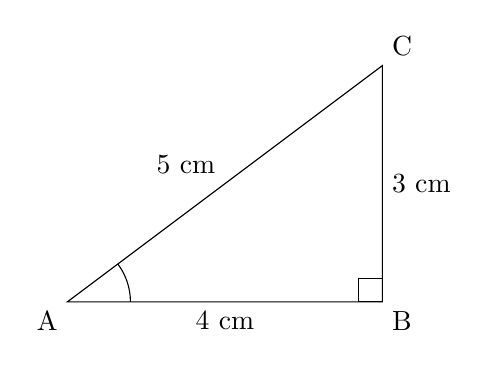
\begin{tikzpicture}
        \coordinate[label=below left:A](A)at(0,0);
        \coordinate[label=below right:B](B)at(4,0);
        \coordinate[label=above right:C](C)at(4,3);
        \tkzMarkRightAngle[size=0.3](C,B,A)
        \tkzMarkAngle[size=0.8,mark=none](B,A,C)
        \draw(A)--(B)--(C)--cycle;
        \path(A)--(B)node[below,midway]{4 cm};
        \path(B)--(C)node[right,midway]{3 cm};
        \path(A)--(C)node[above left,midway]{5 cm};
    \end{tikzpicture}
    \par}\vskip20pt
    cos($\widehat{\text{A}}$) = \vskip50pt
    sin($\widehat{\text{A}}$) = \vskip50pt
    tan($\widehat{\text{A}}$) = \vskip50pt
\end{document}